\begin{frame}{CL ``Compute Device''}
  \begin{columns}
    \column{0.25\textwidth}
      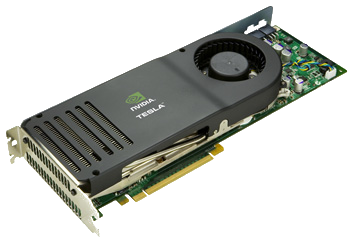
\includegraphics[width=\textwidth]{c870.png}
    \column{0.75\textwidth}
      CL Compute Devices:
      \begin{itemize}
        \item CPUs, GPUs, accelerators, \dots
          \subitem{Anything that fits the programming model.}
        \item A processor die with an interface to off-chip memory
        \item Can get list of devices from platform.
      \end{itemize}
  \end{columns}
\end{frame}
